\documentclass{article}
\usepackage[margin=1in]{geometry} % Set margins to 1 inch on all sides
\usepackage{amsmath, amsfonts, amssymb} % Essential packages for mathematics
\usepackage{graphicx} % For including images
\usepackage{hyperref} % For hyperlinks

\title{The Mathematics of AI and Machine Learning}
\author{Hendrik}
\date{\today}

\begin{document}
	
	\begin{titlepage}
		\newgeometry{margin=1in}
		\centering
		\vspace*{1cm}
		
		{\Huge\bfseries The Mathematics of AI and Machine Learning\par}
		\vspace{1.5cm}
		{\Large\itshape by Hendrik Siemens\par} % "by" added before your name
		\vfill
		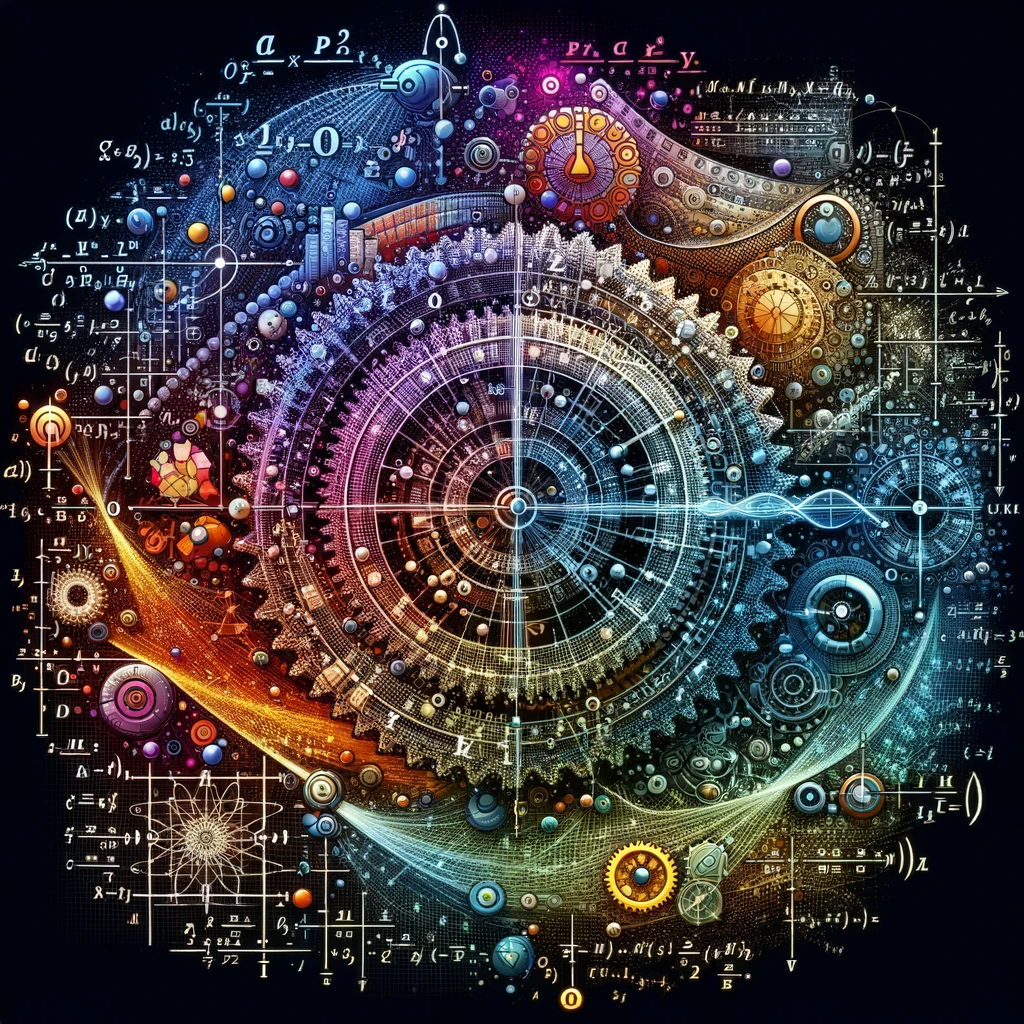
\includegraphics[width=0.9\textwidth]{titel2.png}
		\vfill
		{\Large \today\par}
		\restoregeometry
	\end{titlepage}
	
	\tableofcontents
	\newpage
	
	\section{Introduction}
	\subsection{The Importance of Mathematics in AI and ML}
	% Introduction to why mathematics is crucial in AI and ML
	
	\section{Linear Algebra}
	Linear Algebra is the branch of mathematics concerning linear equations and linear functions which are represented through matrices and vectors. It is central to almost all areas of mathematics and pivotal in machine learning, as it deals with data representations and the transformations applied to them in algorithms.
	
	\subsection{Vectors and Matrices}
	Vectors and matrices are fundamental to the structure of machine learning algorithms. They are used to represent data and operations applied to data.
	
	\subsubsection{Vectors}
	A vector is an ordered finite list of numbers which can represent points in space, and it can also encode various forms of data. For instance, features of a dataset can be encoded as vectors, with each dimension representing a different feature.
	
	\textbf{Definition:}
	A vector in $\mathbb{R}^n$ is a column matrix of n real numbers:
	\[
	\mathbf{v} = \begin{bmatrix}
		v_1 \\
		v_2 \\
		\vdots \\
		v_n
	\end{bmatrix}
	\]
	
	\textbf{Vector Addition:}
	The sum of two vectors is obtained by adding their corresponding entries:
	\[
	\mathbf{u} + \mathbf{v} = \begin{bmatrix}
		u_1 + v_1 \\
		u_2 + v_2 \\
		\vdots \\
		u_n + v_n
	\end{bmatrix}
	\]
	
	\textbf{Scalar Multiplication:}
	A vector can be scaled by a real number, called a scalar. Scalar multiplication involves multiplying each entry of the vector by the scalar:
	\[
	c\mathbf{v} = \begin{bmatrix}
		cv_1 \\
		cv_2 \\
		\vdots \\
		cv_n
	\end{bmatrix}
	\]
	
	\subsubsection{Matrices}
	A matrix is a two-dimensional array of numbers arranged in rows and columns which represents a linear transformation. In machine learning, data is often represented in matrix form.
	
	\textbf{Definition:}
	A matrix with m rows and n columns is an m x n matrix:
	\[
	A = \begin{bmatrix}
		a_{11} & a_{12} & \cdots & a_{1n} \\
		a_{21} & a_{22} & \cdots & a_{2n} \\
		\vdots & \vdots & \ddots & \vdots \\
		a_{m1} & a_{m2} & \cdots & a_{mn}
	\end{bmatrix}
	\]
	
	\textbf{Matrix Multiplication:}
	The product of two matrices is a third matrix where each element is computed as the dot product of corresponding row and column vectors:
	\[
	AB = \begin{bmatrix}
		\sum_{k} a_{1k}b_{k1} & \cdots & \sum_{k} a_{1k}b_{kn} \\
		\vdots & \ddots & \vdots \\
		\sum_{k} a_{mk}b_{k1} & \cdots & \sum_{k} a_{mk}b_{kn}
	\end{bmatrix}
	\]
	
	Matrix multiplication is only possible when the number of columns in the first matrix equals the number of rows in the second matrix.
	
	\subsection{Eigenvalues and Eigenvectors}
	Eigenvalues and eigenvectors are concepts in linear algebra that appear in various data analysis methods. They are pivotal in understanding linear transformations and are used in principal component analysis, a method for dimensionality reduction in machine learning.
	
	\subsubsection{Eigenvalues}
	An eigenvalue is a scalar that determines the factor by which the eigenvector is scaled during a linear transformation.
	
	\textbf{Definition:}
	For a given square matrix \( A \), a non-zero vector \( \mathbf{v} \) is an eigenvector if it satisfies the following equation:
	\[
	A\mathbf{v} = \lambda\mathbf{v}
	\]
	where \( \lambda \) is a scalar known as the eigenvalue corresponding to the eigenvector \( \mathbf{v} \).
	
	The eigenvalues of \( A \) are found by solving the characteristic equation:
	\[
	\det(A - \lambda I) = 0
	\]
	where \( \det \) denotes the determinant of a matrix, and \( I \) is the identity matrix of the same dimension as \( A \).
	
	\subsubsection{Eigenvectors}
	Eigenvectors are vectors that, when a linear transformation is applied, result in the vector being scaled by a factor, which is the eigenvalue. They remain in the same span after the transformation.
	
	\textbf{Computation:}
	For a given eigenvalue \( \lambda \), its eigenvectors are found by solving the equation:
	\[
	(A - \lambda I)\mathbf{v} = 0
	\]
	This equation is solved for the vector \( \mathbf{v} \), giving us the eigenvectors corresponding to \( \lambda \).
	
	\subsection{Singular Value Decomposition}
	Singular Value Decomposition (SVD) is a method of decomposing a matrix into three other matrices and reveals many of the important properties of the original matrix.
	
	\textbf{Definition:}
	Any \( m \times n \) matrix \( A \) can be decomposed as:
	\[
	A = U\Sigma V^*
	\]
	where:
	\begin{itemize}
		\item \( U \) is an \( m \times m \) orthogonal matrix whose columns are the eigenvectors of \( AA^* \).
		\item \( \Sigma \) (often pronounced 'sigma') is an \( m \times n \) diagonal matrix with non-negative real numbers on the diagonal known as the singular values of \( A \).
		\item \( V^* \) (the conjugate transpose of \( V \)) is an \( n \times n \) orthogonal whose columns are the eigenvectors of \( A^*A \).
	\end{itemize}
	
	\textbf{Singular Values:}
	The singular values on the diagonal of \( \Sigma \) are the square roots of the non-negative eigenvalues of \( A^*A \) or \( AA^* \). They are usually arranged in descending order, and the number of non-zero singular values is the rank of matrix \( A \).
	
	\textbf{Application:}
	SVD is widely used in statistics and machine learning for dimensionality reduction, noise reduction, and data compression. It's especially powerful in the context of Principal Component Analysis (PCA) where the eigenvectors correspond to the directions of maximum variance in high-dimensional data, and the singular values are indicative of the importance of each direction.
	
	\textbf{Decomposition Example:}
	To decompose matrix \( A \) using SVD, one must compute:
	\[
	A = U\Sigma V^T
	\]
	Given \( A \) is an \( m \times n \) matrix, \( U \) will be \( m \times m \), \( \Sigma \) will be \( m \times n \), and \( V^T \) (the transpose of \( V \)) will be \( n \times n \).
	
	The columns of \( U \) and \( V \) are orthonormal, and \( \Sigma \) contains the singular values. The matrices \( U \), \( \Sigma \), and \( V \) can be computed using numerical algorithms such as the power iteration or the QR decomposition for large matrices.
	
	\section{Calculus}
	Calculus is the mathematical study of continuous change and it plays an essential role in machine learning for optimizing models and understanding the changes in variables. It is divided into differential calculus, concerning rates of change and slopes of curves, and integral calculus, concerning accumulation of quantities and the areas under and between curves.
	
	\subsection{Differential Calculus}
	Differential Calculus is centered around the concept of the derivative, which measures how a function changes as its input changes. In machine learning, derivatives are crucial for optimization algorithms like gradient descent, as they indicate the direction to adjust model parameters to minimize a loss function.
	
	\subsubsection{Derivative}
	The derivative of a function at a chosen input value describes the rate of change of the function's output with respect to its input value at that point.
	
	\textbf{Definition:}
	The derivative of \( f \) with respect to \( x \) is given by:
	\[
	f'(x) = \lim_{h \to 0} \frac{f(x+h) - f(x)}{h}
	\]
	if this limit exists.
	
	\textbf{Chain Rule:}
	The chain rule is a formula for computing the derivative of the composition of two or more functions:
	\[
	\frac{d}{dx}[f(g(x))] = f'(g(x))g'(x)
	\]
	
	\subsubsection{Gradient}
	In multivariable calculus, the gradient is a multi-dimensional generalization of the derivative and points in the direction of the greatest rate of increase of a function.
	
	\textbf{Gradient Vector:}
	For a function \( f(x, y, ..., z) \), the gradient is a vector of partial derivatives:
	\[
	\nabla f = \begin{bmatrix}
		\frac{\partial f}{\partial x} \\
		\frac{\partial f}{\partial y} \\
		\vdots \\
		\frac{\partial f}{\partial z}
	\end{bmatrix}
	\]
	
	\subsection{Integral Calculus}
	Integral Calculus is concerned with the concept of the integral, which represents the area under a curve and accumulates quantities. In the context of machine learning, integrals are used to calculate the cumulative distribution functions and to understand the total impact of small changes.
	
	\subsubsection{Integral}
	The integral of a function \( f(x) \) over an interval \( [a, b] \) is the net area between the function and the x-axis from \( a \) to \( b \).
	
	\textbf{Definite Integral:}
	The definite integral is given by:
	\[
	\int_{a}^{b} f(x) \, dx
	\]
	which can be interpreted as the accumulated sum of \( f(x) \) values from \( a \) to \( b \).
	
	\textbf{Indefinite Integral:}
	The indefinite integral, or antiderivative, is a function \( F(x) \) whose derivative is \( f(x) \):
	\[
	\int f(x) \, dx = F(x) + C
	\]
	where \( C \) is the constant of integration.
	
	\subsection{Gradient Descent}
	Gradient Descent is a first-order iterative optimization algorithm for finding the minimum of a function. It is a cornerstone of machine learning used to minimize cost functions in model training.
	
	\subsubsection{Algorithm}
	To find a local minimum of a function using gradient descent, one takes steps proportional to the negative of the gradient (or approximate gradient) of the function at the current point.
	
	\textbf{Update Rule:}
	If \( \theta \) is a parameter vector, the update rule is:
	\[
	\theta_{\text{next step}} = \theta - \eta \nabla_\theta J(\theta)
	\]
	where:
	\begin{itemize}
		\item \( \eta \) is the learning rate, a positive scalar determining the size of the step.
		\item \( \nabla_\theta J(\theta) \) is the gradient of the cost function \( J \) with respect to \( \theta \).
	\end{itemize}
	
	\textbf{Learning Rate:}
	The learning rate \( \eta \) is a crucial hyperparameter in gradient descent. If it is too small, the algorithm converges slowly. If it is too large, the algorithm may overshoot the minimum or even diverge.
	
	\textbf{Convergence:}
	The algorithm converges to a local minimum when the gradient \( \nabla_\theta J(\theta) \) is zero, because the update rule no longer changes the parameters.
	
	\textbf{Batch Gradient Descent:}
	The standard form of gradient descent, where the entire dataset is used to compute the gradient at each step.
	
	\textbf{Stochastic Gradient Descent:}
	A variant of gradient descent where one sample from the dataset is used at each iteration. It is much faster and can lead to additional optimization due to its stochastic nature.
	
	\textbf{Mini-Batch Gradient Descent:}
	A compromise between batch and stochastic gradient descent where a subset of the dataset is used at each iteration. It can lead to efficient convergence by balancing the robustness of batch gradient descent and the speed of stochastic gradient descent.
	
	These optimization methods are vital in machine learning to adjust parameters (\( \theta \)) of the model to minimize the cost function \( J \) over the training set.
	% Discuss the role of calculus in optimization and learning algorithms
	
	\section{Probability and Statistics}
	\subsection{Bayesian Thinking}
	\subsection{Probability Distributions}
	\subsection{Statistical Inference}
	% Probability and statistics are foundational to understanding data-driven models
	
	\section{Optimization Theory}
	\subsection{Convex Optimization}
	\subsection{Lagrange Multipliers}
	\subsection{Linear Programming}
	% Optimization theory is critical for training machine learning models
	
	\section{Information Theory}
	\subsection{Entropy}
	\subsection{Information Gain}
	\subsection{Kullback-Leibler Divergence}
	% Information theory concepts applied in machine learning, such as decision trees
	
	\section{Numerical Methods}
	\subsection{Numerical Optimization}
	\subsection{Matrix Factorization}
	\subsection{Root Finding Algorithms}
	% Discuss numerical methods and their applications in machine learning
	
	\section{Conclusion}
	\subsection{The Future of Mathematics in AI and ML}
	% Final thoughts on the evolving role of mathematics in the field
	
\end{document}